\documentclass[10pt]{article}
\usepackage[margin=17mm]{geometry}
\usepackage{graphicx,booktabs,hyperref}
\usepackage[strings]{underscore}
\setlength{\parindent}{0pt}\setlength{\parskip}{5pt}
\begin{document}
\section*{Completed balanced guessing: the registered minima}

Original ell=8, m=3, n=22 Boolean fixtures; fixed prefixes of [7,15,23,24].
The 116 new processes ended at 2026-10-25 17:53:53 UTC; the eight
earlier draw-0/k3 cases remain separate raw records. Of all 124 attempts,
78 refute, 45 saturate without refuting and one is unknown after its 900-second
timeout (draw 6, k=1, branch 1). No missing attempt or zero-cost replacement.

\begin{center}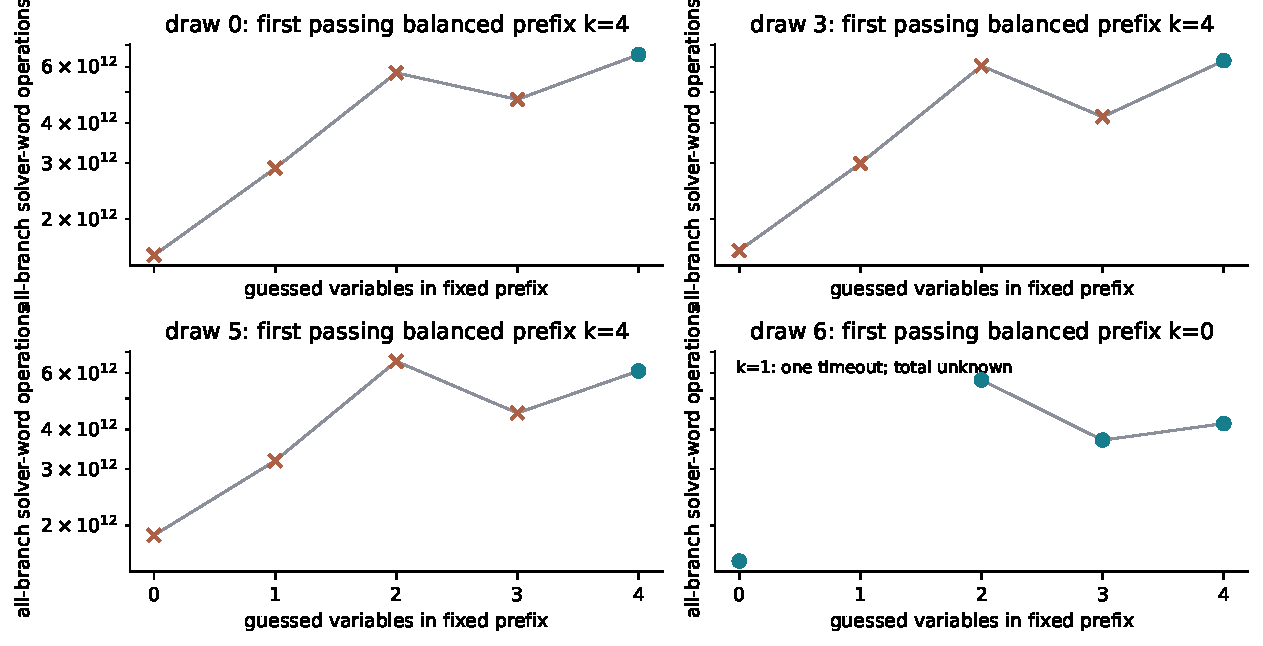
\includegraphics[width=\linewidth]{balanced-prefix-costs.pdf}\end{center}
\begin{center}\small\begin{tabular}{rrrr}\toprule
Draw & First passing k & All passing-set words & Prefix-search words through success\\\midrule
0 & 4 & 6,542,971,204,156 & 21,448,879,433,676 \\
3 & 4 & 6,266,204,429,585 & 21,064,467,554,811 \\
5 & 4 & 6,095,932,567,609 & 22,191,811,097,962 \\
6 & 0 & 1,548,633,051,630 & 1,548,633,051,630 \\
\bottomrule\end{tabular}\end{center}
At k=4 all 64 branches refute, charging 23,078,681,663,212 solver-word
operations across four draws. Every smaller prefix on draws 0,3,5 has
nonrefuting branches, so four is the minimum in this registered prefix family.
Draw 6 refutes at k=0, hence its minimum is zero; the later k=1 timeout is
retained and is irrelevant to that zero lower bound. Green circles indicate
all-branch refutation; crosses indicate a nonrefuting branch; null totals
are missing, never plotted as zero. Prefix-search columns include failed
lower-k work, not just the final passing set. The complete 124-attempt
experimental word total stays unknown because one attempt is censored.

Frozen producer source f83ed00d8, binary SHA prefix ab544a41df94;
input SHA prefix 95ee147e1221. Four Rayon threads, 12-GiB address-space,
900 seconds per new branch, degree four, outer column cap 200,000. Shared
AMD EPYC 9V74 Linux x86-64 host, L0; wall time is diagnostic.
The native completion audit reproduces twice; the complete raw archive
re-extracts byte-identically and its raw-derived summary reproduces.

\textbf{Limits.} This is no minimum over arbitrary variable subsets or
other orderings. It is finite Boolean closure, not a completed ECDLP query.
The explicit reference/twist subgroup gaps and possible cofactor-projected
interpretation remain separate obligations. Independent HKY verdict replay
is genuinely queued after the current m14/15 quartic program; it has not
run and does not independently recount producer words. Construction,
extraction/lifting, verification and native physical prices remain absent.
No full-query/IC/rho or asymptotic claim follows.

\begin{flushleft}\footnotesize
Source: \path{../../pipeline-receipts/guess-completion-20261025-01/summary.json}\par
Complete archive: \path{../../evidence/runs-balanced-guess-complete-all124-20261025.tar.xz}\par
Protocol: COMPLETED_GUESS_REPLAY_PROTOCOL.md; original cap amendment remains
unchanged. No additional paid VM or artifact-store upload is claimed.
\end{flushleft}

\end{document}
